\documentclass{ximera}

\usepackage{graphicx}

\title{A Garden Problem}

\begin{document}

\begin{abstract}
We try to design a garden with the largest possible area - given a fixed length of barbed wire fence.
\end{abstract}

I am building a garden. The amount of stuff I can grow in this garden depends on its \emph{area} - a bigger garden can yield more vegetables. So I'd like the area of my garden to be as large as possible. For simplicity, the garden needs to be rectangular.

However, I also would like to keep deer out of my garden, so I've decided to enclose it with a barbed wire fence. I happen to have 100 meters of barbed wire on hand, and I don't want to buy any more.

\begin{question}
What is the \emph{largest possible} area my garden can have?
\end{question}

Oh - there's one more catch! I've also decided to build the garden so that one side is bordered by a river. Deer don't like to cross this river, so that side doesn't need to have a fence. Here is a rough picture of what the garden will look like: the black lines are barbed wire.

\begin{center}
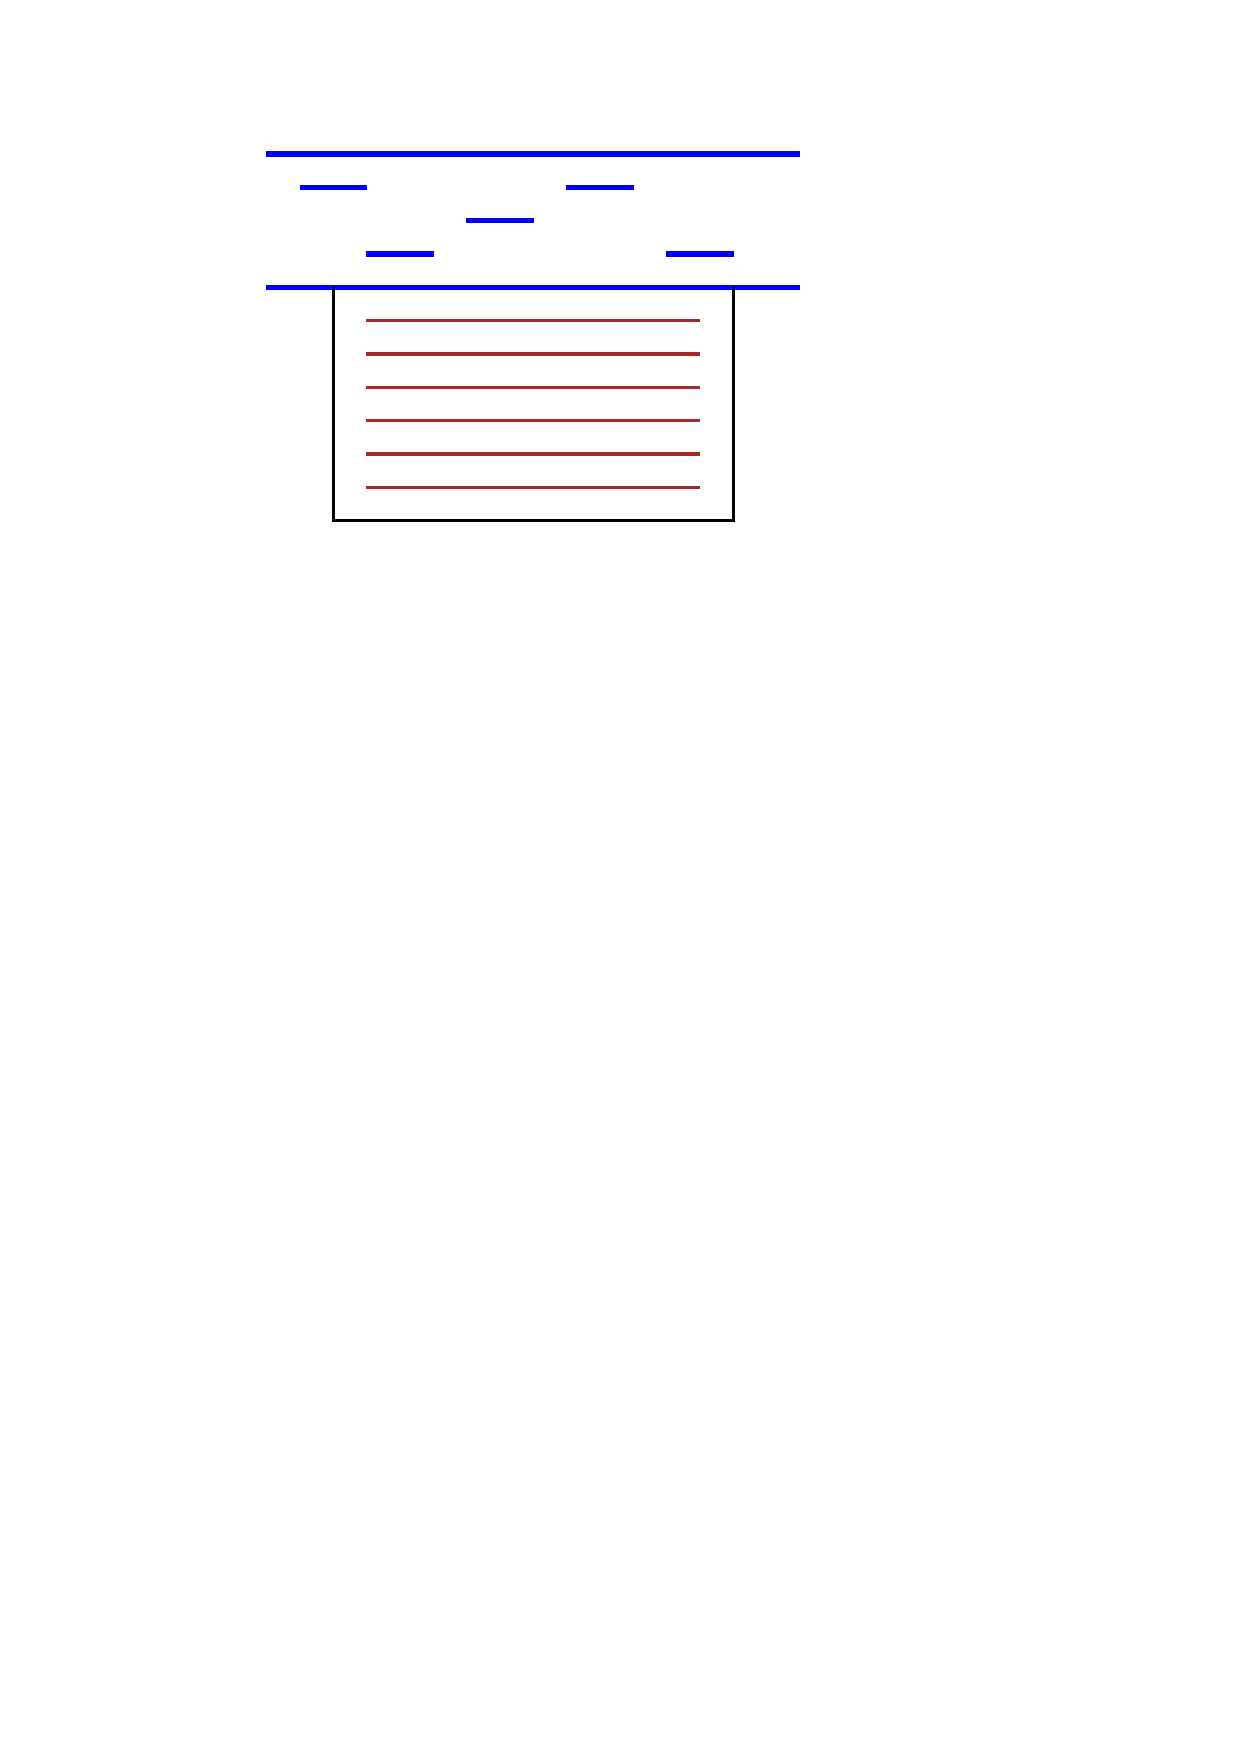
\includegraphics[scale=0.5]{GardenFig}
\end{center}

\begin{exploration}
The length of the rectangle below is automatically changed to reflect changes in the width, $W$. Click and drag point $X$ to see how different values of $W$ affect the rectangle's area.

\geogebra{1445779}{640}{480}
\end{exploration}

\begin{problem}
It appears that the largest possible area is about $\answer[tolerance=5]{1250}$
\end{problem}

\begin{problem}
It appears that the largest area is obtained when $W = \answer[tolerance=1]{25}$
\end{problem}

\end{document}